\chapter{Patchy particle scheme for hydrophilic polymeric networks}

Now that we have covered the theoretical framework, we can delve into the numerical tools that will help us find relations between the polymeric network and the mechanical response.
First, we will describe the patchy particle scheme for simulating PNIPAM cross-linked networks.
Then, we will describe the numerical simulation protocol.
Next, we will introduce the LAMMPS package and explain how it can be used to simulate these systems.
Finally, we will present and analyze the simulation results.

\section{Simulation protocol}

One of the microgels that has been the focus of significant research is the type that is based on PNIPAM cross-linked networks.
In the article \textit{In silico Synthesis of Microgel Particles}\citep{gnanSilicoSynthesisMicrogel2017}, the authors present a flexible numerical protocol capable of designing individual microgel particles based on PNIPAM corr-linked networks. 
This protocol can generate particles with properties comparable to the experimental ones.
In this project, we employ a similar protocol to explore its versatility and identify a numerical tool that can facilitate connections between network configuration and mechanical response.

Our primary focus is on creating networks without spherical confinement and without mimicking the swelling behavior of PINIPAM microgels with temperature.
Therefore, the central strategy involves the implementation of a binary mixture of patchy particles to generate a disorded polymeric network structure, followed by the application of shear deformation.
The primary benefit of this protocol is that previous numerical efforts in microgel modeling have predominantly concentrated on unrealistic networks consisting of chains of equivalent length, frequently establishing cross-linked connections on crystalline lattice regions or where closed polymer networks are assembled by directly integrating randomly dispersed cross-linkers with polymer chains.

\subsection{Patchy particles representation}

A patchy particle\citep{bianchiPhaseDiagramPatchy2006,bianchiTheoreticalNumericalStudy2008} can be defined as a sphere with radius $r$ containing $n$ spheres of radius $l<r$ on its surface.
The smaller spheres are typically referred to as ``patches'' and the number of patches is often refer to as ``functionality''.
The center of the patches can be placed on the surface of the central particle. 
However, it can also be modified to be at a point inside the enclosed volume of the main particle.

The implementation of patchy particles as monomers and crosslinkers is a highly effective strategy.
This is due to the fact that it facilitates the integration of the infinitesimal representation by the Langevin dynamics with a particle that possesses volume and functionality.
The functionality representation is important because it allows for the representation of the monomer and cross-linker molecules that can form a polymeric network.
However, it is important to recognize that the geometry of the monomers and functional groups is assume to be spherical.

Finally, to define the volume of the particle, a repulsive pairwise interaction is defined between the central particles.
Meanwhile, to the formation of a polymeric network is facilitated by an attractive pairwise interaction defined between patches.
Because this model is designed to simulate the final network, not the synthesis process, the pairswise interaction between central particles and patches is not defined.

In contrast, the softness explain by particle interactions is characterized by the form of the repulsive pair potential between two particles.
Finally, the particle volume fraction contributes to the ability of the particles to deform or compress, in contrast to hard spheres\footnote{The patchy particles are hard spheres, but the hydrogel network is a soft ``particle''}\citep{vlassopoulosTunableRheologyDense2014}.

\subsection{Description of the system}

\paragraph{Interaction potentials} We start by describing the interaction potentials between patchy particles.
The interaction between the central particles is modeled with a Weeks-Chandler-Andersen repulsive potential,
\begin{gather}
    U_{WCA}(r_{i,j}) =\left\{ 
        \begin{array}{ll}
            4\epsilon_{i,j}\left[\qty(\frac{\sigma}{r_{i,j}})^{12}-\qty(\frac{\sigma}{r_{i,j}})^6\right]+\epsilon_{i,j}, & r_{i,j}\in[0,2^{1/6}\sigma], \\
            0, & r_{i,j}>2^{1/6}\sigma
        \end{array}
\right.
    ,\label{eqn:CL-MO_interaction}
\end{gather}
where $r_{i,j}$ is the distance between the center of the central particles, $\sigma$ is the diameter of the particles and $\epsilon_{i,j}$ is the energy of the interacton.
On the other hand, the patch-patch interaction is modeled with an attractive potential,
\begin{gather}
    U_{\mathrm{patchy}}\qty(r_{\mu\upsilon}) = \left\{
        \begin{array}{ll}
            2\epsilon_{\mu\upsilon}\left(\frac{\sigma_p^4}{2 r_{\mu\upsilon}^4}-1\right)\exp\left[\frac{\sigma_p}{\qty(r_{\mu\upsilon}-r_{c})}+2\right], & r_{\mu\upsilon}\in\qty[0,r_c], \\
            0, & r_{\mu,\upsilon}>r_c,
        \end{array}
            \right.\label{eqn:patch-patch_interaction}
\end{gather}
where $r_{\mu\upsilon}$ is the distance between two patches, $\sigma_p$ is the diameter of the patches, $r_c$ is the cut distance of interaction set to $1.5\sigma_p$ and $\epsilon_{\mu,\upsilon}$ is the interaction energy between the patches.
This potential can be interpreted as a reversible interaction.

\begin{figure}[ht!]
    \centering
    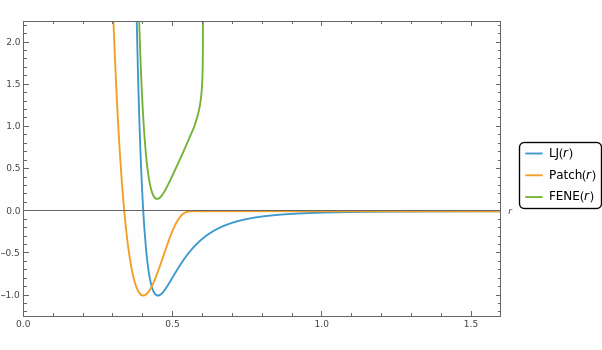
\includegraphics[width=0.8\textwidth]{figs/numerical/patchpatch.png}
    \caption{Comparisson of attractive interaction potentials}\label{fig:patchpatchpot}
\end{figure}

It is important to say that if we let the polymeric network form with only those potentials, the patches are going to form cluster of more then 2 patches, which is not desirble since this will mean that every single monomer can be a crossliker\footnote{Mejorar este enunciado/idea}.
Hence, the interaction between patches is complemented by a three-body repulsive potential, defined in terms of~\eqref{eqn:patch-patch_interaction}, that provides an efficient bond-swapping mechanism making possible to easily equilibrate the system at extremely low temperatures, while at the same time, reataining the single-bond-per-patch condition\citep{sciortinoThreebodyPotentialSimulating2017},
\begin{gather}
    U_{\mathrm{swap}}(r_{l,m},r_{l,n}) = w\sum_{l,m,n}\epsilon_{m,n}U_3\qty(r_{l,m})U_3\qty(r_{l,n}),\quad r_{l,n}\in\qty[0,r_c],\label{eqn:swap_interaction}
\end{gather}
where
\begin{gather}
    U_{3}\qty(r) = \left\{
        \begin{array}{ll}
            1 & r\in\qty[0,r_{\min}], \\
            -U_{\mathrm{patchy}}\qty(r)/\epsilon_{m,n}, & r\in\qty[r_{\min},r_c]
        \end{array}
        \right.\label{eqn:swapmod_interaction}.
\end{gather}
The sum in~\eqref{eqn:swap_interaction} runs over all triples of bonded patches (patch $l$ bonded both with $m$ and $n$).
$r_{l,m}$ and $r_{l,n}$ are the distances between the reference patch and the other two patches.
The parameter $\epsilon_{m,n}$ is the energy of repulsion and $w$ is used to tuned the swapping ($w=1$) and non-swapping bonds ($w\gg1$). 
The cut off distance $r_c$ is the same as in the potential of interaction between patches, meanwhile the minimum distance $r_{\min}$ is the distance at the minimum of~\eqref{eqn:patch-patch_interaction}, \textit{i.e.} $\epsilon_{m,n}\equiv\abs{U_{\mathrm{patchy}}(r_{\min})}$.
Finally, the energy of interaction between crosslinker patches ($\epsilon_{\mu^i,\mu^i}$) are set to $0$ to allow only crosslinker-monomer and monomer-monomer bonding (figure~\ref{fig:intento2}).

\paragraph{Polymeric network parameters}
Now that the interaction between pathcy particles have been described, we can describe the control parameters for the simulations.
We set a constant number of patchy particles $N_p$, a packing fraction $\phi$ and a cross-link concentration $c$. 
From this parameters we compute the volume of the box and the number of patchy particles of functionality 2 (PB) and the patchy particles of functionality 4 (PA).

Due to limitations related to time and computing resources, we have set the total number of particles to be $N_p=\num{8000}$.
This is a lower number of particles when compared with other simulations[cites].
Therefore, in order to compensate, we take the mean of five experiments.
This is equivalent to simulating a system of \num{40000} particles, but with a more manageable computational requirements.

Once we set the parameters for the synthesis, the volume of the box was calculated by determining the volume of the patchy particles A and B, and then scaling those values by the number of particles and the desired packing fraction.
\begin{align*}
    V_{\mathrm{box}} &= \frac{N_{\mathrm{patchyA}}V_{\mathrm{patchyA}}+N_{\mathrm{patchyB}}V_{\mathrm{patchyB}}}{\phi}
\end{align*}
The number of patchy particle of type A is computed as $N_{\mathrm{patchyA}} = c N_p$ and the number of patchy particles of type B as $N_{\mathrm{patchyB}}= N_p - N_{\mathrm{patchyA}}= N_p(1 - c )$.
Finally, the temperature was set to be constant thru all the assembly process $T=0.05$ in Lennard-Jones units, meanwhile, the damp parameter was set to $\mathrm{damp}=0.1$.
It is important to notice that the damp controlls the viscous response from the interaction between the thermal bath and the particles, which represents the interaction between water molecules and the polymer network.

\paragraph{Deformation protocol} 
Once the synthesis of the hydrogel was set, we peform a shear deformation to the resulting polymeric network.
We select the shear deformation because shear forces dominate biological environments where hydrogels are typically deployed. 
Also, shear testing provides a more uniform stress field throughout the hydrogel sample compared to tensile testing. 
In rheological measurements using parallel plate or cone-and-plate geometries, the applied shear stress is distributed evenly across the sample, eliminating edge effects and stress concentrations that plague tensile testing.
Furthermore, shear rheometry excels at characterizing the complex viscoelastic properties that define hydrogel functionality.
Many hydrogels exhibit shear-thinning behavior that is critical for applications like injection and 3D bioprinting. 

Since we are exploring this computational methodology to characterized the mechanical response, we choose to have a constant shear rate to deform beyond the plastic deformation limit.
Also we vary the shear rate of the deformation to see the viscoelastic response of the material.
The temperature was held constant to a value of $0.05$ Lennar-Jones units and a damp on \num{0.1}.


\subsection{LAMMPS implementation}

\paragraph{Three-body potential}
%An importante technica issue to address is the tabulation of the threebody potential to introduce the swap potential into LAMMPS.
This is because the forces on all three particles $I$, $J$, and $K$ of a triplet of this type of three-body interaction potential lie within the plane defined by the three inter-particle distance vectors $\vec{r}_{IJ}$, $\vec{r}_{IK}$ and $\vec{r}_{JK}$.
This property is used to project the forces onto the inter-particle distance vectors.
Hence, we need to create a table taking that into consideration, for that we \textbf{\ldots}

Deformation.

\paragraph{fix deform} To explain how the deformation is perform.

\paragraph{fix stress} to explain how the stress tensor is computed.

\section{Results}

\subsection{Mechanical response}

Strain stress graph

\begin{figure}[ht!]
    \centering
    \includegraphics[width=\textwidth]{figs/ComputaitonalResults/strain-vs-stressxy.png}
    \caption{results from computational results test}
\end{figure}


\subsection{Network analysis}

I guess that figures of the final network and parameter of order or size of porous or whatever.

